\documentclass[tikz,border=5]{standalone}
\usepackage{tikz}
\usetikzlibrary{shapes.geometric, arrows, positioning, fit, calc}



\begin{document}
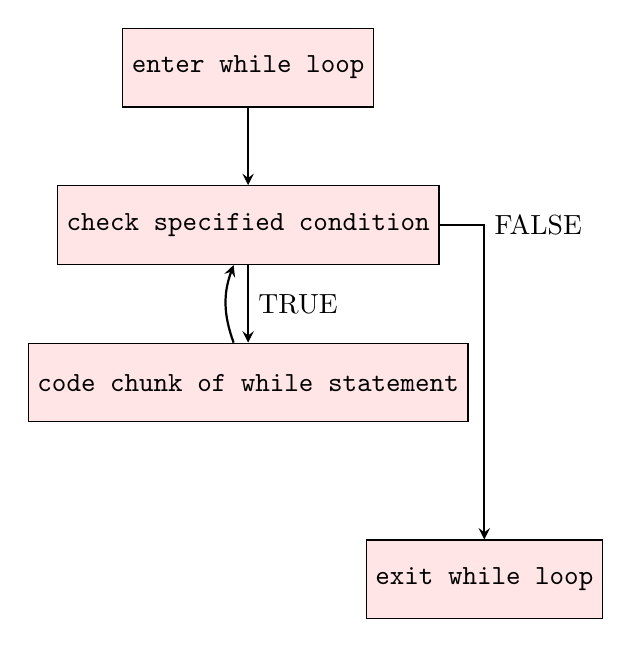
\begin{tikzpicture}
	
	\tikzstyle{chunk} = [rectangle, minimum width=3cm, minimum height=1cm, text centered, draw=black, fill=red!10]
	\tikzstyle{arrow} = [thick,->,>=stealth]
	
	\node (enter) [chunk] at (12,4.5) {\texttt{enter while loop}};
	\node (check) [chunk] at (12,2.5) {\texttt{check specified condition}};
	\node (code) [chunk] at (12,0.5) {\texttt{code chunk of while statement}};
	\node (exit) [chunk] at (15,-2) {\texttt{exit while loop}};
	
	\draw [arrow] (enter) -- (check);
	\draw [arrow] (check) -| node[right] {FALSE} (exit);
    \draw[arrow] (check) -- node[right] {TRUE} (code);
    \draw[arrow] (code) to[bend left=20]  (check);
 
\end{tikzpicture}
\end{document}